\chapter{绪论}

\section{引言}
\subsection{流变学的核心研究内容}
流变学是研究物质在外力作用下变形和流动的科学,其研究对象涵盖了流体、软固体以及在特定条件下可以流动的固体\cite{dealyIntroductionRheology1990}。流变学的核心在于揭示材料的应力、应变和时间之间的内在关系,并通过本构方程(流变状态方程)对这些关系进行定量描述。流变学的研究不仅深化了对材料力学行为的理解,还为工程应用和科学研究提供了重要的理论基础。流变学的核心研究内容主要包括以下几个方面\cite{elleroTanner90Years2024}:
\begin{enumerate}[topsep = 0 pt, itemsep= 0 pt, parsep=0pt, partopsep=0pt, leftmargin=44pt, itemindent=0pt, labelsep=6pt, label=(\arabic*)]
	\item 材料的流动与变形行为:材料的流动与变形行为是流变学研究的核心内容之一。通过实验和理论模型,流变学揭示了材料在外力作用下的复杂力学行为。例如,蠕变现象(即在恒定应力下,材料的变形随时间逐渐增加)和应力松弛现象(即在恒定应变下,材料的应力随时间逐渐减小)是流变学中重要的研究对象。这些现象不仅反映了材料的时间依赖性行为,还为材料的长期性能评估提供了理论依据。此外,流变学还研究了材料的非线性力学行为,如屈服、塑性变形和断裂等,这些研究对于理解材料的宏观力学性能具有重要意义。
	\item	  本构方程的构建:本构方程是流变学中用于描述材料力学行为的数学工具,其核心在于建立应力、应变和时间之间的定量关系。对于牛顿流体,其本构方程基于牛顿黏性定律,即应力与应变率成正比。然而,对于非牛顿流体和软固体,其本构方程则更为复杂,通常需要考虑材料的非线性、黏弹性以及时间依赖性等特性。通过构建合理的本构方程,流变学能够对各种物理现象进行精确的数学描述,从而为工程设计和材料开发提供理论支持。
	\item  实验与模拟方法:流变学实验是研究材料流变性能的重要手段,常见的实验方法包括蠕变实验、应力松弛实验和动力试验等。这些实验能够直接测量材料在不同条件下的力学响应,为理论模型的验证和优化提供实验数据。近年来,随着计算模拟技术的发展,流变学研究逐渐从唯象模型向定量科学转变。微观实验技术(如X射线散射、中子散射)与计算模拟的结合,使得研究者能够在微观尺度上揭示材料的流变机制,从而推动流变学向更高精度和更深层次发展。
\end{enumerate}
\subsection{流变学应用方向}
流变学的研究方向广泛,涵盖了多个学科和领域,例如高分子流变学研究高分子材料的分子结构与其流变行为的关系,例如聚合物熔体和溶液的拉伸流变行为。生物流变学研究生物材料(如血液、肌肉)的流变特性,揭示生理和病理过程中的力学机制。地质流变学研究岩石、土壤等地质材料的流变行为,应用于地震预测、矿产资源开发等领域。工业流变学在材料加工、食品工业、化妆品和医药制造等领域,流变学用于优化工艺和产品性能。非牛顿流体力学研究不符合牛顿黏性定律的流体(如油漆、泥浆、血液)的流动特性。

\section{本构方程}
\subsection{线性本构方程}
凝聚相物质分为固体或液体,固体和液体之间的一个区别特征是它们对施加的力的响应。固体在变形时储存能量,如果变形很小,则在消除力后会恢复到原来的形状。相比之下,液体则会通过耗散能量和调整其形状来抵抗力\cite{ricarteTutorialReviewLinear2024}。这种区别可以通过两种经典的力学模型来描述:胡克固体(Hookean Solid) 和牛顿流体(Newtonian Fluid)。胡克定律(Hooke's Law) 可以来描述小变形下的弹性固体行为。胡克定律表明,固体的应力$\sigma$与应变$\gamma$成正比,如公式\eqref{eq:hookean_solid}所示。其中,$G$为弹性模量,用于描述材料在弹性变形范围内抵抗外力的能力。它反映了材料的刚度,即材料在受力时发生变形的难易程度。弹性模量越大,材料越难变形;弹性模量越小,材料越容易变形。胡克固体是理想化的弹性固体模型,适用于描述金属、陶瓷等材料在小变形条件下的力学行为。
\begin{equation}
	\sigma = G \gamma  \label{eq:hookean_solid}
\end{equation}
而对于液体,其对外力的响应则完全不同。液体无法储存能量以恢复形状,而是通过内部的粘性阻力来耗散能量,并持续流动以适应外力。这种行为可以用牛顿流体的本构方程来描述,即剪切应力与剪切速率成正比,如公式\eqref{eq:newton_fluid}所示。其中,$\eta$为粘性系数,用于描述液体在运动过程中耗散能量的能力。粘性系数越大,液体越容易耗散能量,反之亦然。牛顿流体是理想化的粘性流体模型,适用于描述水、空气等液体在运动过程中耗散能量的行为。
\begin{equation}
	\sigma = \eta \dot{\gamma}  \label{eq:newton_fluid}
\end{equation}
然而,这些特征都是理想化的,代表了特定条件的行为。许多凝聚相材料不容易归入这些经典类别,因为它们的机械性能取决于变形的大小、速率、变形历史,加载过程等等。例如,考虑牙膏,它像液体一样流动,可以将其从管中挤出,但一旦放在牙刷上,它就会像固体一样保持其形状。这类物质同时具有黏性和弹性,被认为是黏弹性材料,被称为软物质或者复杂流体。

线性黏弹性理论认为在小变形范围(线性范围内)应力-应变关系是线性的,即应力与应变成正比。同时线性黏弹性区间内材料具有时间依赖性,材料的力学响应不仅取决于当前的应力或应变,还依赖于时间或加载历史。
\begin{figure}[htbp]
	\centering
	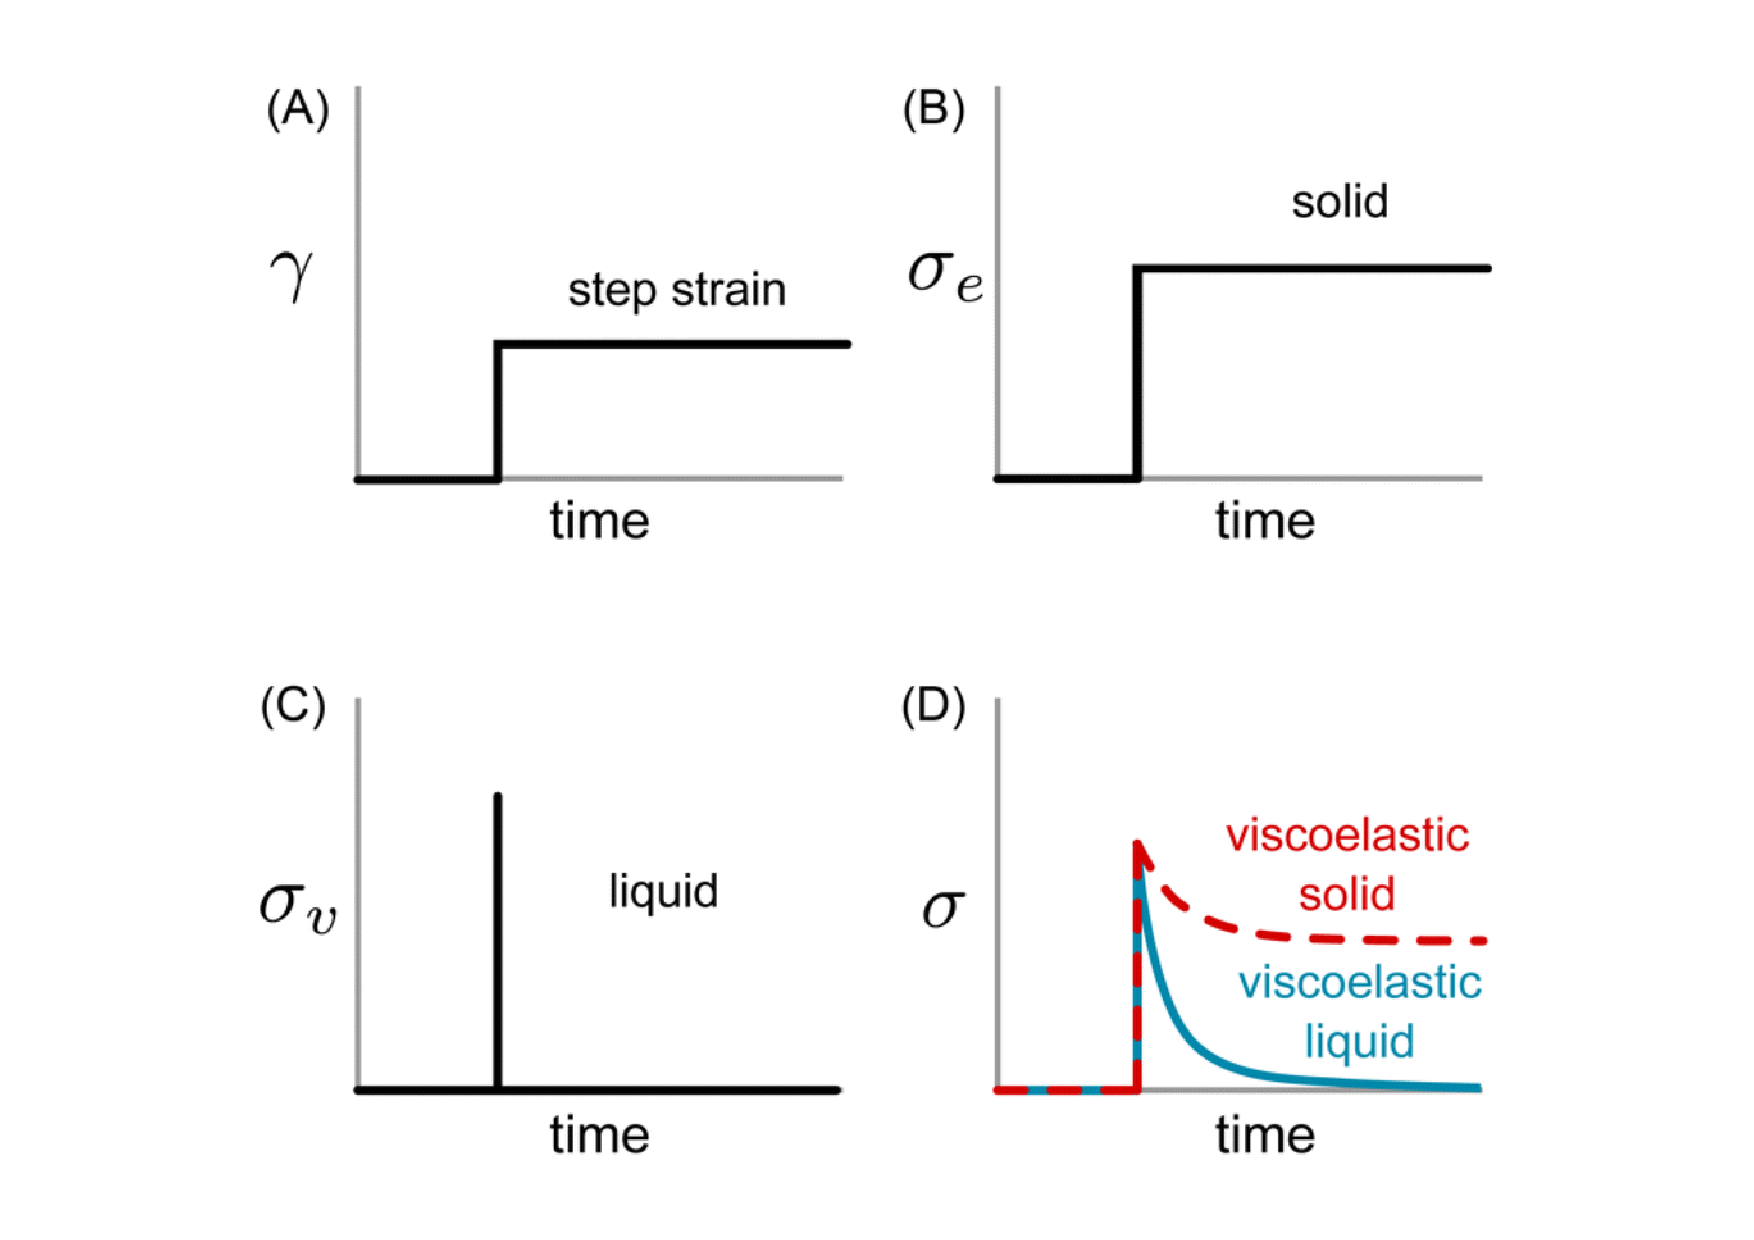
\includegraphics[width=\textwidth]{Fig/solid_liquid.pdf}
	\FigureBicaption{\label{differ_fluid_intro}(A)施加的应变曲线以及对应的剪切应力;(B)理想弹性固体;(C)理想粘性液体;(D)粘弹性样品\cite{ricarteTutorialReviewLinear2024}}{(A) Applied strain profile and resulting shear stress;(B) ideal elastic solid;(C) ideal viscous liquid;(D) viscoelastic samples\cite{ricarteTutorialReviewLinear2024}}
\end{figure}
图\ref{differ_fluid_intro}概述了两种不同类型的粘弹性材料的简单剪切行为。对于粘弹性固体和液体,阶跃应变会引起瞬时弹性响应,从而产生σ峰值。然而,应力不是保持不变或立即降至零,而是逐渐降低。它在很长一段时间内接近粘弹性固体的有限平台值,而粘弹性液体则完全衰减到零\cite{ricarteTutorialReviewLinear2024}。

线性本构理论中最经典的是Maxwell模型,如图\ref{maxwell_intro}所示,Maxwell模型将材料的弹性行为和粘性行为结合起来,它用一个弹簧(弹性元件)和一个粘壶(粘性元件)串联表示黏弹性关系。Maxwell模型的微分形式如公式\eqref{eq:maxwell_model_dt}所示,其中$\tau$表示松弛时间,等于$eta/G$。将两边积分得到Maxwell模型的积分形式如公式\eqref{eq:maxwell_model_int}所示。
\begin{align}
	 & \frac{d\sigma}{dt} + \frac{\sigma}{\tau}  = G \frac{d\gamma}{dt} \label{eq:maxwell_model_dt}                                                   \\
	 & \sigma(t)                                = \int_{-\infty}^{t} G e^{-\frac{t-t'}{\tau}} \frac{d\gamma(t')}{dt'} dt'\label{eq:maxwell_model_int}
\end{align}
积分形式的方程显示了任何时刻的应力是松弛模量乘以应变速率的积分,该时刻之前材料的整个历史。由于被积函数中的衰减指数,模型具有衰落的记忆,因此最近的应变历史比过去的应变历史更重要。
\begin{figure}[htbp]
	\centering
	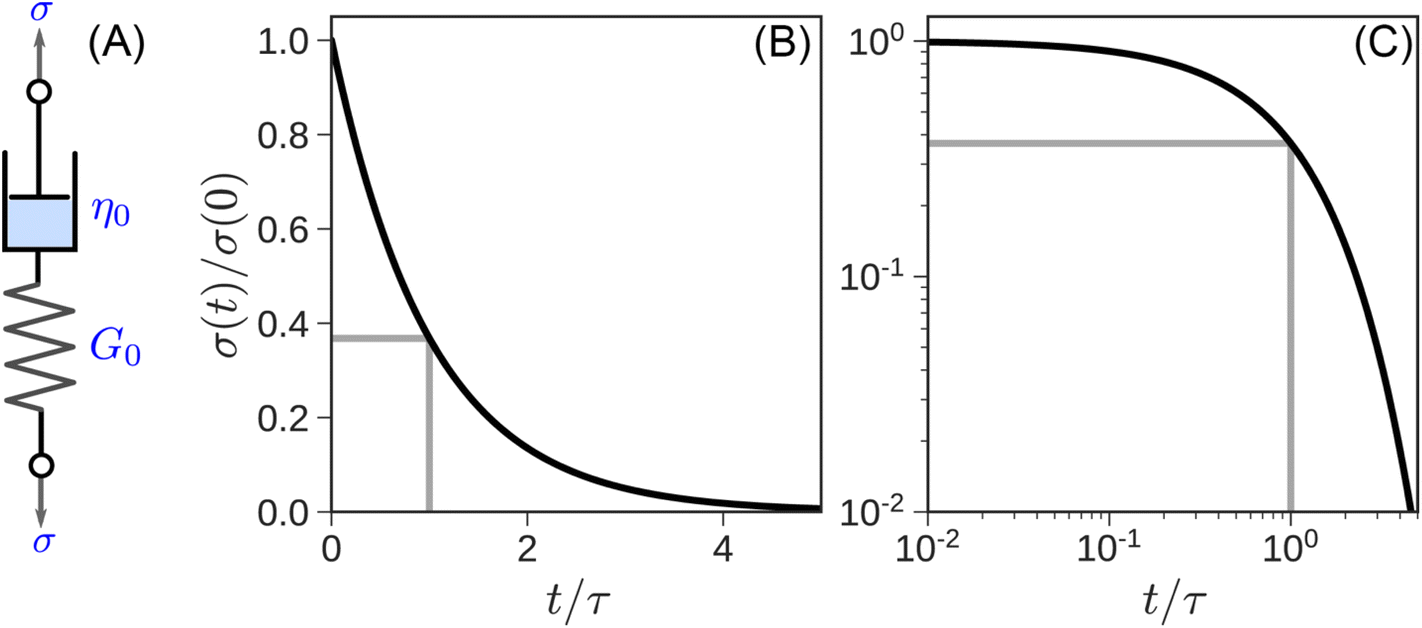
\includegraphics[width=0.8\textwidth]{Fig/maxwell_intro.png}
	\FigureBicaption{\label{maxwell_intro} Maxwell 模型示意图}{Maxwell model schematic}
\end{figure}
如果将多个Maxwell模型并联,便可以得到广义Maxwell模型方程,如公式\eqref{eq:generalized_maxwell_model}所示。
\begin{equation}
	\sigma(t) = \int_{-\infty}^{t} G(t-t') \frac{d\gamma(t')}{dt'} dt' \label{eq:generalized_maxwell_model}
\end{equation}
其中松弛模量 \(G(t)\) 定义为公式\eqref{eq:generalized_maxwell_model_G}。
\begin{equation}
	G(t) = \sum_{i=1}^{n} G_i e^{-\frac{t}{\tau_i}} \label{eq:generalized_maxwell_model_G}
\end{equation}

Maxwell模型通过将黏弹性抽象为黏性元件和弹性元件串联来得到本构方程。如果将弹簧和粘壶进行并联,则得到Kelvin-Voigt 模型的本构方程。
\subsection{非线性本构方程}
\subsection{传统的本构方程的构建方法}

\section{机器学习理论}
\subsection{传统机器学习方法}
\subsection{神经网络与深度学习}
\subsection{注意力机制}
\subsection{生成式模型}

\section{深度学习应用于本构方程研究现状}
\subsection{纯数据驱动方法}
\subsection{引入物理约束的神经网络研究}

\section{本课题研究介绍}
\subsection{研究内容}
\subsection{创新之处}
\subsection{研究意义}



